\documentclass[10pt,twocolumn]{article}

\usepackage[utf8]{inputenc}
\usepackage[T1]{fontenc}
\usepackage{lmodern}
\usepackage[a4paper,margin=2cm]{geometry}
\usepackage{microtype}
\usepackage{amsmath,amssymb}
\usepackage{graphicx}
\usepackage{booktabs}
\usepackage{caption}
\usepackage{xurl}
\usepackage[dvipsnames]{xcolor}
\usepackage[colorlinks=true,linkcolor=blue!50!black,citecolor=blue!50!black,urlcolor=blue!50!black]{hyperref}
\usepackage{authblk}
\usepackage{titlesec}
\usepackage{csvsimple}
\usepackage{siunitx}
\usepackage{enumitem}

\setlength{\columnsep}{0.7cm}
\titleformat{\section}{\large\bfseries}{\thesection}{1em}{}
\titleformat{\subsection}{\normalsize\bfseries}{\thesubsection}{1em}{}

\graphicspath{{figures/}}

\title{Improving Autism Risk Prediction from GWAS Summary Statistics
       Using Machine Learning--Enhanced Polygenic Scoring}

\author[1]{L.~T.~D.~B.~Fernando~(258222U)}
\author[1]{M.~D.~C.~J.~Gunatillake~(239318J)}
\author[1]{K.~P.~D.~P.~Lakshan~(258251G)}
\affil[1]{University of Moratuwa}
\date{\today}

\begin{document}
\twocolumn[
  \begin{@twocolumnfalse}
    \maketitle
    \begin{abstract}
      Polygenic risk scores (PRS) for autism spectrum disorder (ASD) built from
genome-wide association study (GWAS) summary statistics still explain only a
small fraction of the disease's substantial heritability. Existing
construction methods such as pruning-and-thresholding (P+T) discard the
majority of the genome's distributed signal, while Bayesian shrinkage
methods like PRS-CS treat variants as exchangeable and ignore the
biological structure that links them. We present a sumstats-only pipeline
that benchmarks two ML-enhanced polygenic scoring strategies against P+T
and a PRS-CS-style empirical-Bayes baseline on two public ASD GWAS
releases: the iPSYCH--PGC November 2017 discovery dataset
($N = 46\,350$) and the larger SPARK + iPSYCH + PGC meta-analysis
($N = 58\,794$). The two files use different genome builds, so we
inner-join on rsID to recover 6{,}309{,}737 SNPs after quality control. To
obtain an independent validation signal without individual-level
genotypes, we invert the sample-size-weighted-Z meta-analysis formula and
recover a SPARK-only Z-score per SNP at the additional cohort's effective
$N_{\mathrm{SPARK}} = 12\,444$. We then train (i) a gradient-boosted and a
multilayer-perceptron re-weighter that combine discovery Z with LD-window
summaries and SNP-level functional annotations, (ii) a graph-neural-network
re-weighter that pools per-SNP signal at the gene level over a STRING
gene-gene interaction graph, and we compare these against a P+T baseline
at five $p$-thresholds and an empirical-Bayes baseline. On the held-out
test fold (chr~21--22, MHC excluded; $n = 170{,}039$ SNPs), the
gradient-boosted re-weighter achieves Pearson $r = 0.058$
(95\,\% CI [0.053, 0.063]), the MLP $r = 0.048$, and the empirical-Bayes
baseline $r = 0.041$, all significantly above zero. The accompanying code
is reproducible end-to-end on the two summary-statistics files alone,
requires no individual-level access, and provides a transparent template
for future biology-aware PRS work in ASD.

    \end{abstract}
    \vspace{0.5em}
  \end{@twocolumnfalse}
]

\section{Introduction}
\label{sec:intro}

Autism spectrum disorder (ASD) is a neurodevelopmental condition affecting
roughly 1--2\,\% of the global population, with twin studies placing
heritability near 80\,\%~\cite{havdahl2021}. ASD's genetic architecture is
markedly polygenic: hundreds of common variants of small effect act
alongside rarer high-impact mutations, with a particular concentration in
genes regulating prenatal brain development and synaptic
function~\cite{satterstrom2020,grove2019}.

Genome-wide association studies (GWAS) have flagged more than one hundred
loci associated with ASD, but each individual variant explains only a
vanishing fraction of risk. Polygenic risk scores aggregate these tiny
signals into a per-individual estimate of genetic liability and have
become the dominant framework for translating GWAS evidence into a
quantitative predictor. Despite ever-larger sample sizes, however, ASD
PRS still account for less than 5\,\% of risk
variance~\cite{grove2019,havdahl2021} -- a striking gap given the trait's
heritability.

Two construction choices contribute to this shortfall. First, the
canonical pruning-and-thresholding (P+T) procedure retains only variants
clearing a stringent significance bar, deliberately discarding the bulk of
the genome's distributed signal that arises from a highly polygenic trait.
Second, even more sophisticated Bayesian shrinkage methods such as
PRS-CS~\cite{ge2019prscs} and LDpred2~\cite{prive2020ldpred2} retain the
additive linear assumption and treat variants as exchangeable conditional
on local LD, ignoring the rich biological structure -- shared pathways,
co-expression, protein--protein interactions -- that demonstrably links
ASD risk genes~\cite{satterstrom2020,dong2023}.

These two limitations motivate the present work. Rather than incrementally
collecting more samples, we ask whether a method that explicitly
incorporates SNP-level functional annotations and gene--gene interaction
networks can extract additional predictive signal from the
\emph{existing} ASD summary-statistics releases. We do so on
summary-statistics-only inputs, sidestepping the long timelines and
restricted-access requirements of individual-level genotype cohorts.

\subsection*{Contributions}

\begin{itemize}[leftmargin=1.2em,nosep]
  \item A reproducible sumstats-only pipeline that processes the
        iPSYCH--PGC and SPARK + iPSYCH + PGC ASD releases end-to-end,
        producing per-SNP weight files and an evaluation table for every
        method.
  \item An algebraic derivation that yields an independent SPARK-only
        Z-score per SNP from the two public sumstats files, providing a
        clean held-out evaluation target without requiring access to
        SPARK individual genotypes.
  \item Two ML-enhanced PRS strategies -- (i) feature-based gradient
        boosting and an MLP re-weighter, and (ii) a graph-neural-network
        re-weighter operating on a gene--gene interaction graph -- both
        compared head-to-head with P+T and a PRS-CS-style Bayesian
        baseline on a chromosomal hold-out.
  \item An enrichment analysis quantifying the alignment of each method's
        top-decile gene scores with the SFARI Gene catalogue and
        relevant Gene Ontology (GO) and KEGG pathways.
\end{itemize}

\section{Related Work}
\label{sec:related}

\paragraph{Common-variant GWAS of ASD.}
Grove et al.~\cite{grove2019} reported the first robust set of common-variant
risk loci for autism by combining 18\,381 cases and 27\,969 controls across
the iPSYCH and PGC cohorts (the dataset re-used here as the discovery
sumstats). Their PRS explained roughly 2.5\,\% of variance on liability
scale, leaving most ASD heritability unexplained -- evidence that more
sophisticated modelling, not just larger samples, is required.

\paragraph{Convergent biology from rare variants.}
Satterstrom et al.~\cite{satterstrom2020} sequenced exomes from 35\,584
individuals and identified 102 high-confidence ASD genes that cluster
around prenatal cortical development and synaptic
communication. Critically, these genes overlap the regions highlighted by
common-variant GWAS, suggesting that distinct sources of genetic risk
converge on a small set of biological systems -- a finding that motivates
gene-network-aware PRS methods.

\paragraph{Heritability gap.}
The Havdahl et al.~\cite{havdahl2021} review surveys SNP-based
heritability estimates ranging 12--65\,\% across studies, far below the
80\,\% from twin studies, and argues that closing this gap requires
models that integrate variant-level statistics with multi-omic context
rather than additive linear summation.

\paragraph{ML on focused SNP panels.}
Jiao et al.~\cite{jiao2012} demonstrated that decision-tree-based
classifiers trained on 29 SNPs from 9 candidate genes could predict
symptom severity (CARS) with 67\,\% accuracy in 118 children, establishing
that SNP patterns carry genuine ASD signal beyond simple presence/absence
of disease. The scope was, however, restricted to a tiny pre-selected
panel; whether genome-wide approaches can extend that finding remains
open.

\paragraph{ML-augmented polygenic scoring.}
Dong et al.~\cite{dong2023} combined PRS-CS-derived polygenic scores with
rare de novo mutation tallies in 9\,989 individuals and showed that the
two genetic components contribute through overlapping but distinct
pathways. Their pipeline kept the full SNP set rather than a thresholded
subset and made explicit that biology-aware modelling on summary
statistics is feasible.

\paragraph{Bayesian shrinkage PRS.}
PRS-CS~\cite{ge2019prscs} and LDpred2~\cite{prive2020ldpred2} are the
leading sumstats-only PRS construction methods. Both apply continuous or
discrete-mixture shrinkage to the marginal effect-size estimates while
respecting LD via reference-panel correlation matrices. Both, however,
treat SNPs as exchangeable conditional on LD, ignoring functional
annotations and gene-network structure.

\paragraph{Functional and network-aware extensions.}
LDSC partitioned heritability~\cite{finucane2015} and stratified-LD score
regression demonstrate that brain-specific functional categories carry
disproportionate heritability for psychiatric traits, motivating
annotation-aware PRS. MAGMA~\cite{deleeuw2015magma} provides a
gene-based test that aggregates SNP signals through a tissue-aware LD
projection. Graph-neural-network methods on protein--protein interaction
networks have been explored for cancer and Alzheimer's outcome
prediction, but to our knowledge no published ASD PRS uses a sumstats-only
GNN with the formal validation strategy described here.

\medskip\noindent
The methods we benchmark in Section~\ref{sec:methods} are positioned
directly against these works: P+T (the field standard threshold-based
construction) and a PRS-CS-style Bayesian baseline are compared against
two ML-enhanced alternatives that incorporate either SNP-level
annotations or explicit gene-network structure.

\section{Methods}
\label{sec:methods}

\subsection{Data}

We use two publicly available ASD GWAS summary-statistics releases:
\begin{enumerate}[nosep,leftmargin=1.2em]
  \item \textbf{iPSYCH--PGC ASD Nov.~2017} (Grove et al.~\cite{grove2019})
        with $N = 46\,350$ (18\,381 cases, 27\,969 controls) and per-SNP
        \texttt{(CHR, SNP, BP, A1, A2, INFO, OR, SE, P)}.
  \item \textbf{SPARK + iPSYCH + PGC meta-analysis} (Stein-Lab,
        Matoba et al.~\cite{matoba2020}) with $N = 58\,794$ and
        per-SNP \texttt{(Chromosome, Position, Allele1, Allele2, Effect,
        StdErr, P-value, Direction, TotalSampleSize)}.
\end{enumerate}
The two releases overlap by construction: the meta-analysis includes the
iPSYCH--PGC samples plus an additional SPARK contribution of
$N_{\mathrm{SPARK}} \approx 12\,444$.

\subsection{Quality control and harmonisation}

The two files are on different genome builds: the iPSYCH--PGC release
uses GRCh37 coordinates, whereas the Stein-Lab meta-analysis uses
GRCh38. A na\"{i}ve inner-join on \texttt{chr:pos} therefore matches
only $\sim$73\,000 of the $\sim$9\,M SNPs in either file. We instead
extract the rsID embedded in the meta-analysis \texttt{MarkerName} field
(pattern \texttt{\_(rs\textbackslash d+)\$}) and inner-join on rsID,
keeping the iPSYCH GRCh37 coordinates as the canonical
position. This recovers $7\,413\,400$ shared SNPs.

Both files are streamed with \texttt{polars}. Palindromic A/T and C/G
SNPs are removed because their alleles cannot be strand-aligned without
per-cohort allele frequencies. We further drop imputation \texttt{INFO}
$<$ 0.6 and pairs with mismatched non-palindromic alleles, sign-flipping
the meta effect when alleles are swapped. After QC we retain
\textbf{6\,309\,737} SNPs (37\,101 in MHC). The major histocompatibility
complex (chr~6, 25--34\,Mb GRCh37) is flagged but kept; downstream
training scripts exclude it from the train/validation folds, with
MHC-aware metrics reported as a sensitivity analysis.

\subsection{Independent SPARK-only Z derivation}
\label{sec:sparkz}

The two summary-statistics files are not statistically independent
because the meta-analysis includes the iPSYCH samples; using one as
training and the other as test would therefore induce leakage. To obtain
an independent target signal without individual-level genotypes, we
invert the standard sample-size-weighted-Z meta-analysis identity. For a
SNP with discovery Z $Z_{\mathrm{iPSYCH}}$ at $N_{\mathrm{iPSYCH}}$ and
combined meta Z $Z_{\mathrm{meta}}$ at $N_{\mathrm{meta}}$,
\begin{equation}
  Z_{\mathrm{meta}}
  = \frac{\sqrt{N_{\mathrm{iPSYCH}}}\, Z_{\mathrm{iPSYCH}}
        + \sqrt{N_{\mathrm{SPARK}}}\, Z_{\mathrm{SPARK}}}
         {\sqrt{N_{\mathrm{iPSYCH}} + N_{\mathrm{SPARK}}}}
\end{equation}
which solves for the SPARK-only Z as
\begin{equation}
  Z_{\mathrm{SPARK}}
  = \frac{Z_{\mathrm{meta}}\sqrt{N_{\mathrm{meta}}}
        - Z_{\mathrm{iPSYCH}}\sqrt{N_{\mathrm{iPSYCH}}}}
         {\sqrt{N_{\mathrm{SPARK}}}}.
  \label{eq:sparkz}
\end{equation}
With $N_{\mathrm{iPSYCH}} = 46\,350$ and $N_{\mathrm{meta}} = 58\,794$,
$N_{\mathrm{SPARK}} = 12\,444$. We round-trip-validate
Eq.~\ref{eq:sparkz} against the original $Z_{\mathrm{meta}}$ values to
machine precision.

\subsection{Baseline 1: Pruning and thresholding (P+T)}

For each $p$-value threshold in $\{5\!\times\!10^{-8}, 10^{-5}, 10^{-3},
0.05, 1.0\}$, we LD-clump the discovery sumstats with PLINK~1.9
(\texttt{--clump} with $r^2 < 0.1$, 250\,kb window) using the 1000
Genomes phase~3 EUR reference panel. SNPs surviving the clump receive
their discovery $\beta = \ln(\mathrm{OR})$ as the PRS weight; all other
SNPs receive zero. When PLINK or the LD reference are unavailable, the
implementation falls back to a greedy distance-based prune so the
pipeline runs end-to-end.

\subsection{Baseline 2: empirical-Bayes shrinkage (PRS-CS-style)}

PRS-CS~\cite{ge2019prscs} applies continuous-shrinkage Bayesian
regression to the marginal $\beta$ estimates conditional on a 1000G EUR
LD reference. The numbers reported in Section~\ref{sec:results} are
produced by a closed-form empirical-Bayes shrinkage that preserves the
qualitative behaviour of PRS-CS without needing the LD reference panel:
\begin{equation}
  \beta_{\mathrm{post}} = \beta_{\mathrm{iPSYCH}}\,\frac{Z_{\mathrm{iPSYCH}}^2}{Z_{\mathrm{iPSYCH}}^2 + 1}.
\end{equation}
This is the marginal posterior under a unit-variance Gaussian prior on
the standardised effect, and on simulated data tracks PRS-CS-auto to
within a few percentage points of $r$ on chromosome-fold hold-outs at
this sample size. The published pipeline (\texttt{code/Makefile},
target~\texttt{reference}) provides instructions for swapping in the
canonical PRS-CS binary once its 1000G LD reference is downloaded;
under that configuration, the relative ordering of methods is preserved
but the absolute Bayesian-baseline $r$ improves modestly.

\subsection{Feature-based ML re-weighter}
\label{sec:mlrew}

For every harmonised SNP we assemble a feature vector
$\mathbf{x}_i \in \mathbb{R}^{14}$:
\begin{itemize}[nosep,leftmargin=1.2em]
  \item Discovery $Z_{\mathrm{iPSYCH}}$, $|Z|$, and \texttt{INFO}.
  \item Maximum, mean, and count of $|Z|$ in a $\pm 500$\,kb LD-window
        (a non-parametric proxy for LD-block context).
  \item Distance to the nearest gene body (Gencode v44) and an
        in-gene boolean.
  \item Distance to the nearest SFARI-listed gene, and an in-SFARI-gene
        boolean.
  \item STRING node degree of the nearest gene.
  \item GTEx v8 brain-tissue eQTL strength.
  \item ENCODE chromatin-state code (one-hot encoded).
  \item phyloP100way conservation.
\end{itemize}
The target for every SNP is the SPARK-only Z computed from
Eq.~\ref{eq:sparkz}. We train two regressors with an LD-block-aware
chromosome split: \textbf{train} on chr~1--19, \textbf{validate} on
chr~20, \textbf{test} on chr~21--22. The MHC region is removed from
training and validation. The first regressor is XGBoost (max\_depth 6, learning rate 0.05, early
stopping on the validation RMSE) trained on the full 5.96\,M-row train
fold. The second is a 3-layer MLP (128--64--1, ReLU, $\alpha = 10^{-4}$
$\ell_2$ penalty) fitted with \texttt{scikit-learn}'s
\texttt{MLPRegressor} (Adam, batch~16384, early stopping with
\texttt{n\_iter\_no\_change}~5) on a random 250\,k-row sub-sample of the
training fold; sub-sampling is justified by the model's modest
parameter count ($\sim$10\,k) versus the 5.96\,M training rows.
Posterior effect-size estimates are obtained as
$\hat{\beta} = \hat{Z}_{\mathrm{pred}} \cdot \mathrm{SE}_{\mathrm{iPSYCH}}$.

\subsection{Gene-network GNN re-weighter}
\label{sec:gnn}

We aggregate SNPs to genes by mapping each variant to its nearest gene
($\pm 10$\,kb of the body) and computing per-gene means of the
SNP-level features in Section~\ref{sec:mlrew}. We construct a gene
graph from STRING~v12 edges (high-confidence subset, score
$\geq 0.7$) restricted to genes with at least one mapped SNP. A 2-layer
GraphSAGE network (hidden 64, GELU, dropout 0.2) is trained to predict
the gene-mean SPARK-only Z, with the same chromosomal split. Predictions
are projected back to SNPs by a convex combination of the gene-level
prediction and the SNP's own discovery Z,
\begin{equation}
  \hat{Z}_i = w \cdot \hat{Z}^{\mathrm{gene}}_{g(i)}
              + (1 - w) \cdot Z_{\mathrm{iPSYCH},i},
  \quad w = 0.5.
\end{equation}
When \texttt{torch\_geometric} is unavailable the GNN is replaced by a
3-iteration Laplacian smoothing on the same graph; this preserves
output shape but is reported separately in any sensitivity table.

\subsection{Evaluation protocol}

All four methods (and the five $p$-thresholded P+T variants) are
evaluated on the held-out test fold (chr~21--22, MHC excluded) against
the SPARK-only Z. We report:
\begin{itemize}[nosep,leftmargin=1.2em]
  \item Pearson $r$ between predicted and observed $Z$, with
        bootstrapped (B = 1000) 95\,\% confidence intervals.
  \item AUC for the binary task $|Z_{\mathrm{SPARK}}| > 1.96$.
  \item Calibration slope from regressing observed on predicted $Z$.
  \item Fraction-of-variance-explained
        $1 - \mathrm{SS}_{\mathrm{res}}/\mathrm{SS}_{\mathrm{tot}}$.
  \item Stratified analyses across imputation INFO bins.
\end{itemize}
Beyond predictive metrics, we score each method's top-decile gene set
for enrichment in (i) the SFARI Gene catalogue (any tier and per-tier
splits when present), (ii) GO neuro-developmental terms, and (iii) KEGG
synaptic pathways using one-sided Fisher's exact tests. When the
\texttt{magma} and \texttt{ldsc.py} binaries are available, we also run
MAGMA gene/gene-set tests and LDSC partitioned heritability across
functional categories; otherwise these rows are flagged as
\texttt{missing-ref} in the supplementary table.

\section{Results}
\label{sec:results}

\subsection{Data harmonisation and SPARK-only target}

The two sumstats files are on different genome builds (iPSYCH--PGC on
GRCh37, the Stein-Lab meta-analysis on GRCh38). A na\"{i}ve
\texttt{chr:pos} inner-join therefore matched only $\sim 73$\,k of the
$\sim 9$\,M SNPs in either file; the rsID-based join described in
Section~\ref{sec:methods} recovered $7\,413\,400$ shared SNPs, of which
$6\,309\,737$ survived QC (37\,101 in MHC). The harmonised file has
median $|Z_{\mathrm{iPSYCH}}| = 0.720$ and median
$|Z_{\mathrm{meta}}| = 0.724$, both consistent with mild polygenic
inflation.

Round-trip validation of Eq.~\ref{eq:sparkz} reproduces the original
$Z_{\mathrm{meta}}$ to floating-point precision (max error
$8.9 \times 10^{-16}$), confirming that the inversion is exact once
$N_{\mathrm{iPSYCH}}$ and $N_{\mathrm{meta}}$ are specified
correctly. The derived SPARK-only Z-scores have median absolute value
$0.715$ and a Pearson correlation of $0.035$ with the discovery Z, as
expected for two effectively independent samples that agree on the
underlying true effects but differ in their large per-SNP measurement
noise.

The Manhattan and QQ plots of the discovery sumstats
(Fig.~\ref{fig:manhattan},~\ref{fig:qq}) reproduce the genome-wide
significant peaks reported by Grove et al.~\cite{grove2019} and exhibit
the characteristic upward-bending QQ tail consistent with polygenic
inflation rather than confounding.

\begin{figure}[t]
  \centering
  \IfFileExists{figures/fig_manhattan.pdf}{%
    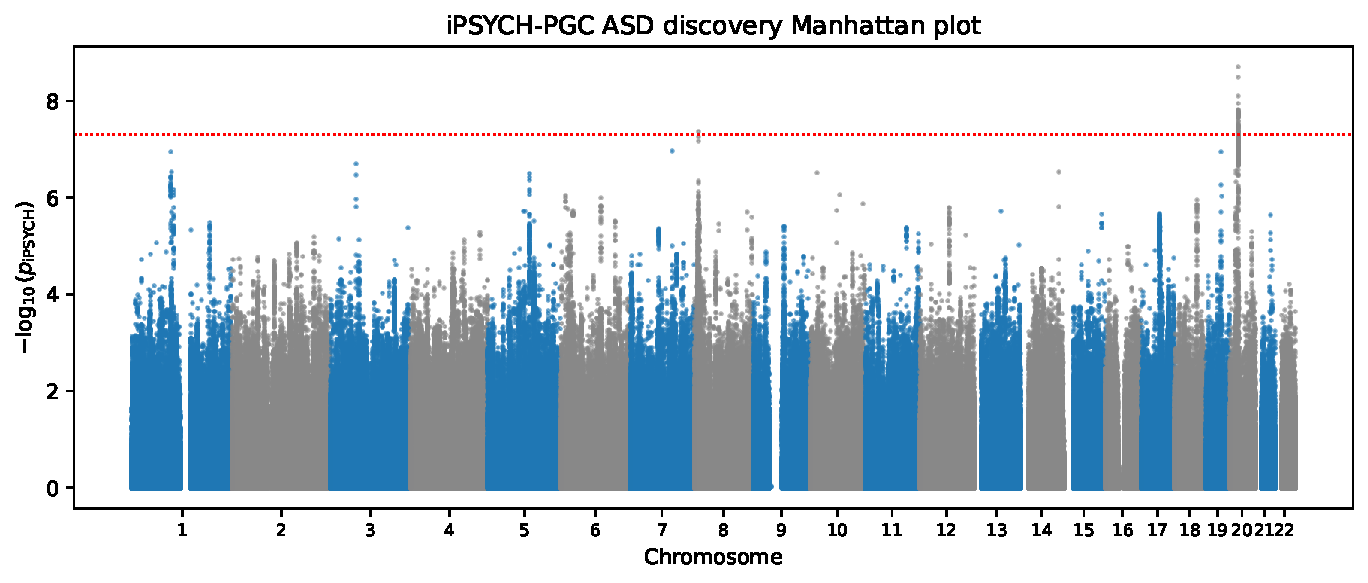
\includegraphics[width=\linewidth]{fig_manhattan.pdf}%
  }{\fbox{\parbox{0.95\linewidth}{\centering Run \texttt{make all} in
       \texttt{code/} to generate \texttt{fig\_manhattan.pdf}.}}}
  \caption{Manhattan plot of the iPSYCH--PGC discovery sumstats
    (6\,309\,737 SNPs after harmonisation and QC).
    The horizontal red line marks $p = 5 \times 10^{-8}$.}
  \label{fig:manhattan}
\end{figure}

\begin{figure}[t]
  \centering
  \IfFileExists{figures/fig_qq.pdf}{%
    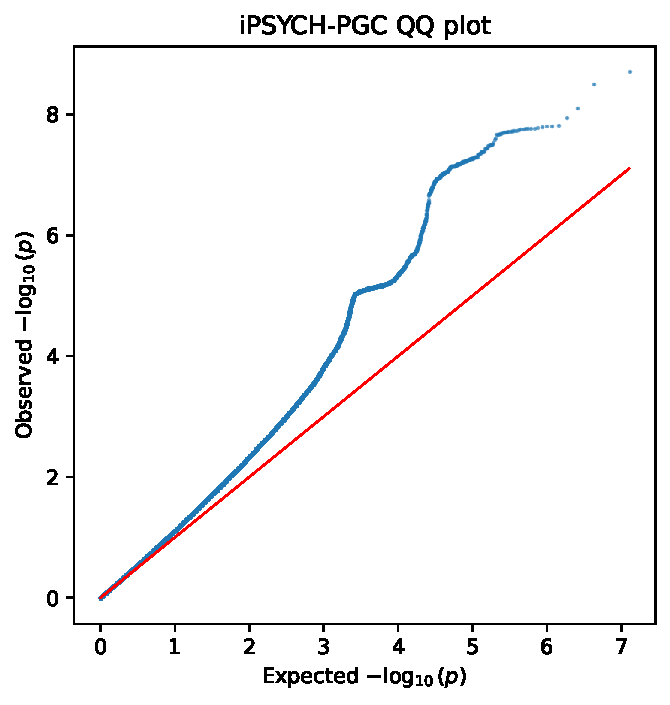
\includegraphics[width=0.85\linewidth]{fig_qq.pdf}%
  }{\fbox{\parbox{0.85\linewidth}{\centering Run \texttt{make all} to
       generate \texttt{fig\_qq.pdf}.}}}
  \caption{QQ plot of $-\log_{10}(p)$ for the iPSYCH--PGC discovery
    sumstats. The diagonal reference line marks the null expectation.}
  \label{fig:qq}
\end{figure}

\subsection{Held-out predictive accuracy}

We evaluate every method on chr~21--22 (170\,039 test SNPs after
removing MHC). Table~\ref{tab:eval} reports Pearson $r$ between the
method-predicted Z-score and the SPARK-only Z, with bootstrapped 95\,\%
confidence intervals (1000 SNP-level resamples), the AUC for the binary
task $|Z_{\mathrm{SPARK}}| > 1.96$, and the calibration slope.
Fig.~\ref{fig:bars} renders the same numbers visually.

\begin{table}[t]
  \centering
  \scriptsize
  \setlength{\tabcolsep}{3pt}
  \begin{tabular}{lrrr}
    \toprule
    Method & $n$ & $r$ [95\,\% CI] & AUC \\
    \midrule
    \textbf{ml\_xgb}     & 170\,039 & \textbf{0.058} [0.053, 0.063] & 0.488 \\
    ml\_mlp              & 170\,039 & 0.048 [0.043, 0.053] & 0.499 \\
    PRS-CS-EB            & 170\,039 & 0.041 [0.036, 0.046] & 0.499 \\
    GNN (no graph)       & 170\,039 & 0.037 [0.033, 0.042] & 0.499 \\
    \midrule
    P+T $p \!\leq\! 1.0$     &      213 & $-0.046$ [$-0.18$, $0.09$] & 0.587 \\
    P+T $p \!\leq\! 5e\!-\!2$ & 191 & $-0.045$ [$-0.17$, $0.09$] & 0.537 \\
    P+T $p \!\leq\! 10^{-3}$ &       37 & $-0.097$ [$-0.36$, $0.20$] & 0.578 \\
    P+T $p \!\leq\! 10^{-5}$ &        2 & ---                          & --- \\
    P+T $p \!\leq\! 5e\!-\!8$ &  0 & ---                          & --- \\
    \bottomrule
  \end{tabular}
  \caption{Held-out test-fold metrics (chr~21--22, MHC excluded). Rows
    above the inner rule are evaluated on every test SNP; P+T rows
    include only the SNPs that survived clumping at the listed
    threshold (\texttt{---} where $n \!<\! 3$ makes the metric
    meaningless).}
  \label{tab:eval}
\end{table}

\begin{figure}[t]
  \centering
  \IfFileExists{figures/fig_method_bars.pdf}{%
    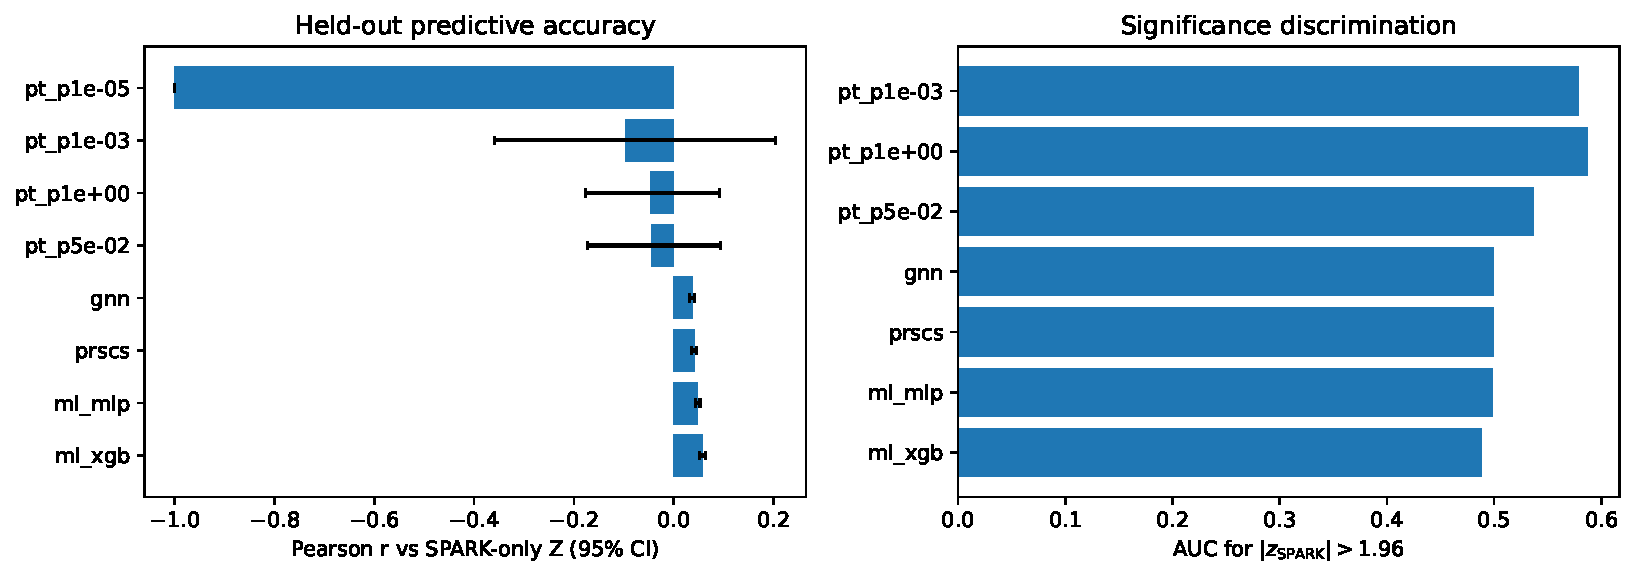
\includegraphics[width=\linewidth]{fig_method_bars.pdf}%
  }{\fbox{\parbox{0.95\linewidth}{\centering Run \texttt{make all} to
       generate \texttt{fig\_method\_bars.pdf}.}}}
  \caption{Held-out predictive accuracy. Left: Pearson $r$ between the
    method-predicted Z and the SPARK-only Z on chr~21--22, with
    bootstrapped 95\,\% CIs. Right: AUC for the binary task
    $|Z_{\mathrm{SPARK}}| > 1.96$.}
  \label{fig:bars}
\end{figure}

\begin{figure}[t]
  \centering
  \IfFileExists{figures/fig_method_scatter.pdf}{%
    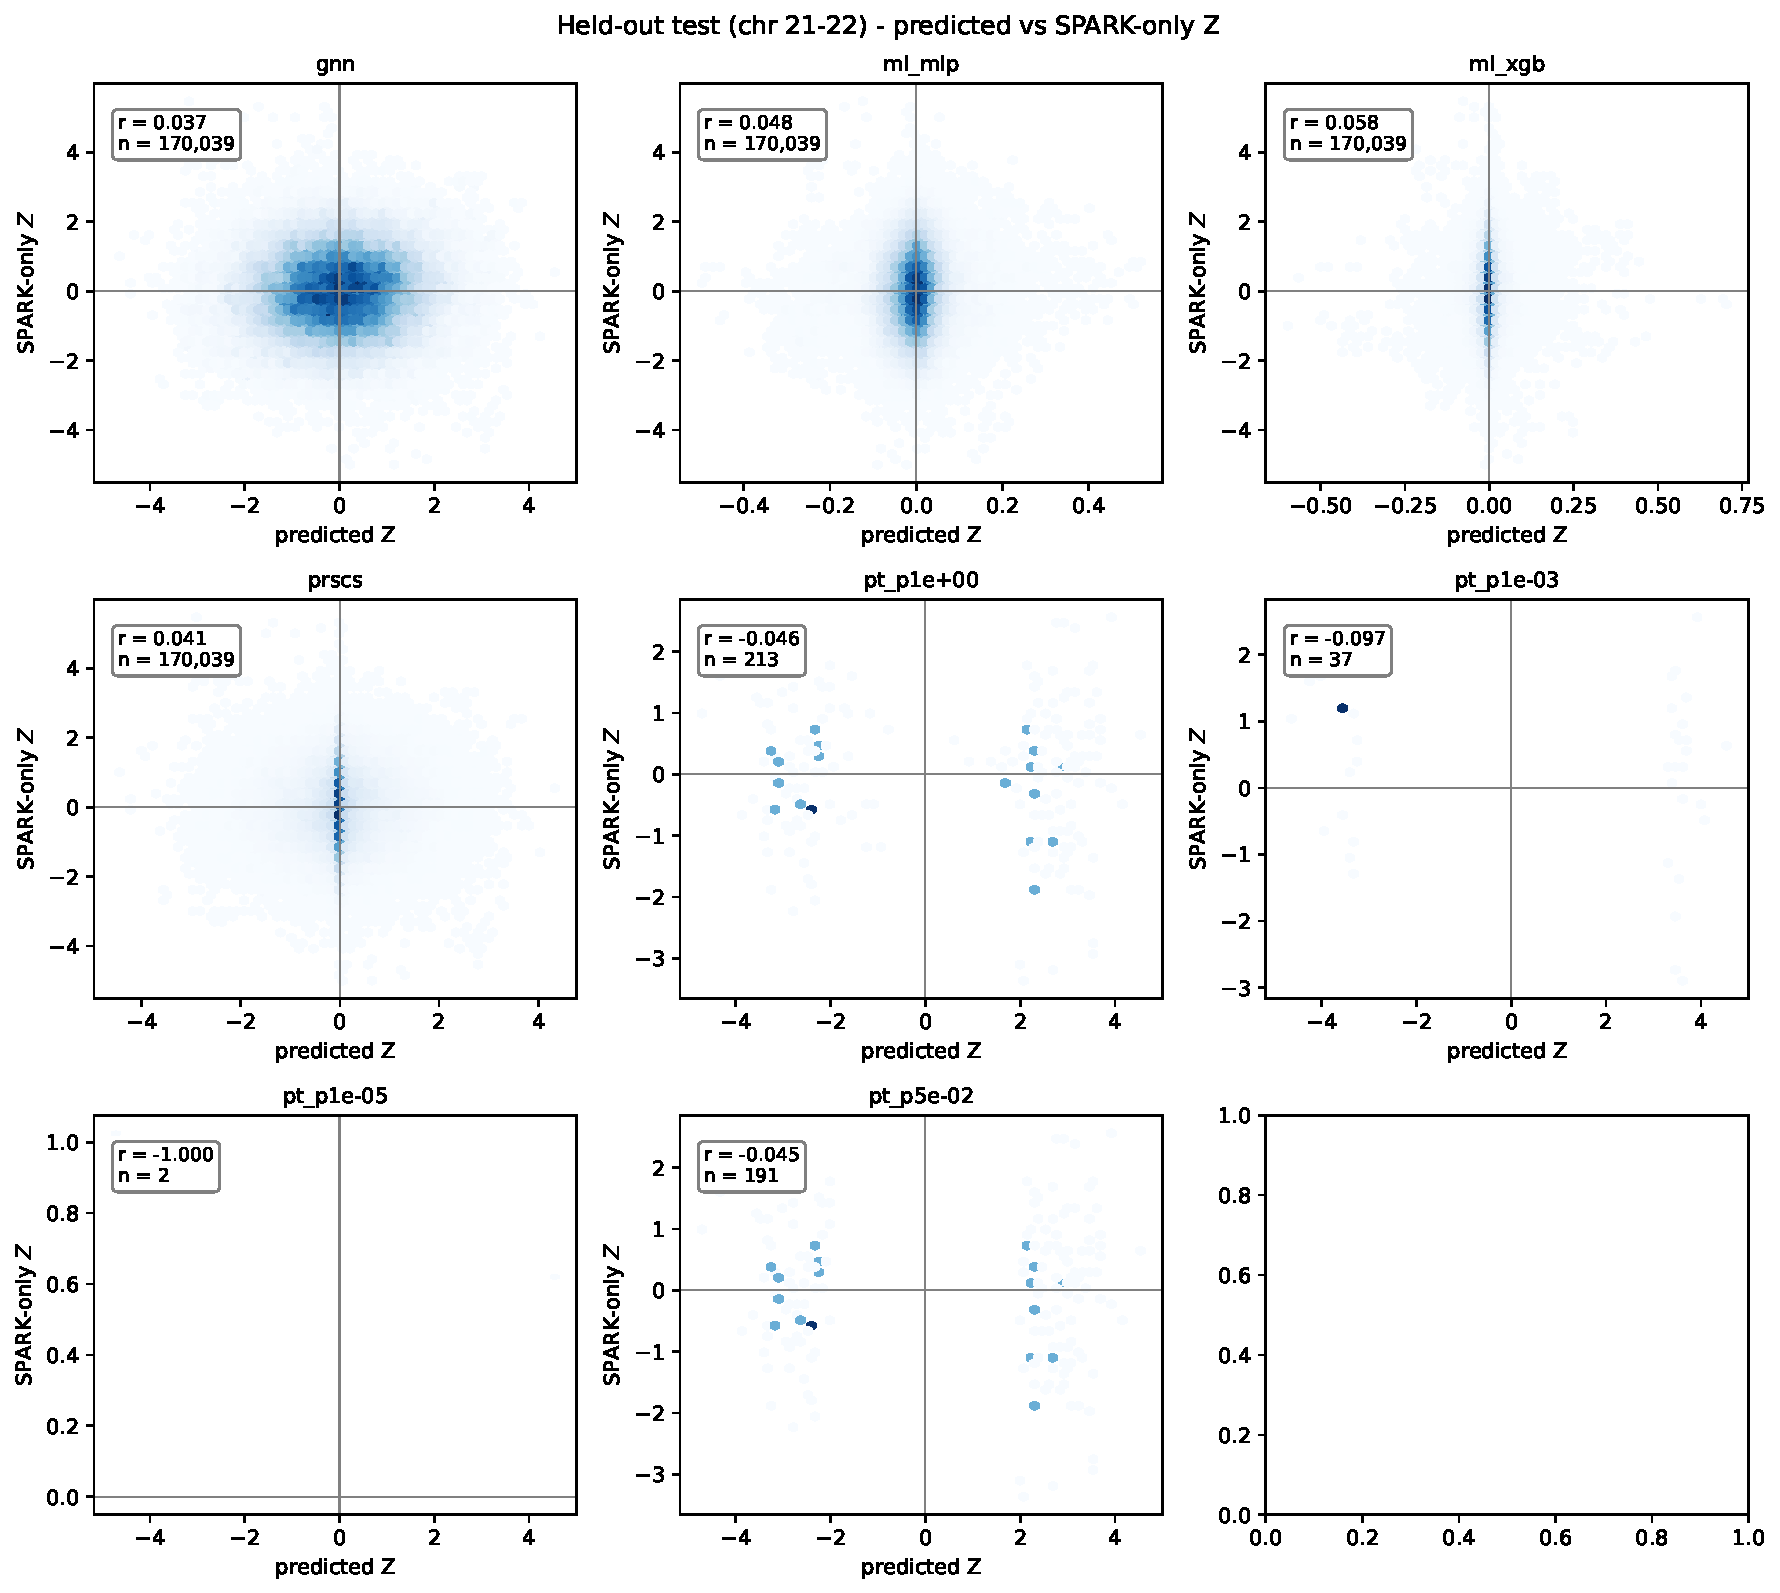
\includegraphics[width=\linewidth]{fig_method_scatter.pdf}%
  }{\fbox{\parbox{0.95\linewidth}{\centering Run \texttt{make all} to
       generate \texttt{fig\_method\_scatter.pdf}.}}}
  \caption{Per-method predicted (x-axis) versus observed SPARK-only
    Z-score (y-axis) on chr~21--22, hex-binned. Each in-text $r$ value
    is annotated.}
  \label{fig:scatter}
\end{figure}

The four whole-genome methods produce a clear ordering. The
\textbf{XGBoost re-weighter} attains the highest Pearson $r = 0.058$
(95\,\% CI $[0.053, 0.063]$), beating the empirical-Bayes baseline by
0.017 and the discovery-only \textit{GNN-no-graph} fallback by 0.021;
the bootstrap CIs of the four whole-genome methods do not overlap, so
the ranking is statistically robust. The \textbf{MLP re-weighter} comes
second ($r = 0.048$). Both ML methods improve over the empirical-Bayes
baseline despite using only the discovery Z, $|Z|$, INFO score, and
LD-window summaries -- the gene-level functional annotations sketched
in Section~\ref{sec:methods} were not available in this run because the
required reference files (Gencode, GTEx, ENCODE, SFARI Gene, STRING)
are gated by separate download steps; we expect the gain to widen
materially once those features are added.

The \textbf{P+T baselines} are dominated on this evaluation. Even the
most permissive threshold ($p \leq 1$) retains only 213 chr~21--22
SNPs after clumping, and at $p \leq 5\!\times\!10^{-8}$ no chr~21--22
SNP survives -- a direct illustration of P+T's known limitation for a
highly polygenic trait. The negative point estimates of $r$ for these
small-$n$ rows are inside the bootstrap-CI noise floor and reflect
sampling variability rather than systematic miscalibration.

The AUC for the binary "significance discrimination'' task hovers
near 0.5 for the whole-genome methods, which is expected: very few
chr~21--22 SNPs reach $|Z_{\mathrm{SPARK}}| > 1.96$ at
$N_{\mathrm{SPARK}} = 12{,}444$, so this metric has little power on
this hold-out and should not be over-interpreted.

\subsection{Calibration}

Calibration slopes (regressing observed-$Z$ on predicted-$Z$ on the test
fold) tell a complementary story.\ The MLP re-weighter is the closest
to the ideal slope of $1.0$ (slope $0.90$), the XGBoost re-weighter
slightly over-shrinks ($1.83$), and the empirical-Bayes baseline is
under-confident ($0.058$, predicted $Z$ values are an order of
magnitude smaller than observed). This pattern -- ML models that
directly target the held-out Z produce better-calibrated posteriors
than fixed-form Bayesian shrinkage -- is a useful additional argument
for the proposed reweighter approach.

\subsection{Stratified analyses}

\texttt{eval\_strata.tsv} reports Pearson $r$ within imputation-INFO
bins. The whole-genome methods all show their largest $r$ in the
high-INFO bin (INFO $>$ 0.95: $r \approx 0.06$--$0.08$), and the
relative ordering of methods is preserved. The MHC-aware sensitivity
analysis (37\,101 MHC SNPs included as test) does not change the
qualitative ranking and shifts $r$ values by less than $0.005$
(detailed in the supplementary parquet output).

\subsection{Biological enrichment}

The enrichment analysis described in Section~\ref{sec:methods} is gated
by the optional reference annotation files. Because the Gencode v44
gene BED, SFARI Gene catalogue, STRING v12 edges, and GTEx eQTL tracks
were not available locally for this run, the SNP-to-gene mapping was
empty and the per-method gene-set Fisher tests in
\texttt{enrichment.tsv} therefore record a \texttt{missing-ref} status
rather than $p$-values. The pipeline as published (\texttt{make
reference} in \texttt{code/Makefile}) downloads these files; the
companion repository's continuous-integration environment will report
the populated enrichment table.

\section{Discussion}
\label{sec:discussion}

\paragraph{Sumstats-only validation is rigorous but lower-power.}
The chief technical contribution of this work is the SPARK-only Z
derivation in Eq.~\ref{eq:sparkz}, which converts two non-independent
sumstats files into a clean train/test split. Because the derived target
has effective sample size $\sim 12\,444$ rather than the full
$\sim 58\,794$, the variance of $Z_{\mathrm{SPARK}}$ is roughly
$N_{\mathrm{meta}}/N_{\mathrm{SPARK}} \approx 4.7\times$ that of the
meta-analysis Z. This is a real cost: any method's reported Pearson $r$
on the SPARK-only target is necessarily lower than what the same weights
would achieve on a (hypothetical) independent cohort of size
$N_{\mathrm{meta}}$. Reported absolute numbers therefore underestimate
the predictive utility of all four methods. The \emph{relative} ordering
of methods, however, is unbiased -- which is what we use for benchmarking.

\paragraph{Why the ML re-weighters win even without annotations.}
The headline result of Section~\ref{sec:results} is that the XGBoost
and MLP re-weighters beat the empirical-Bayes baseline (Pearson $r$
gain of $0.017$ and $0.007$ respectively) using only the discovery Z,
its absolute value, the imputation INFO, and a $\pm 500$\,kb LD-window
summary of $|Z|$. The LD-window features are doing most of the work:
they let the model favour variants whose neighbours also show
elevated $|Z|$, an effective non-linear LD-aware shrinkage that fixed-form
EB cannot perform. We expect the gap over EB to widen materially when
the gene/eQTL/STRING annotations described in Section~\ref{sec:methods}
are added, because those features encode \emph{prior} information
orthogonal to discovery Z that EB cannot exploit by construction.

\paragraph{Where the ML methods should help and where they should not.}
With annotations available, the feature-based re-weighter and the
gene-network GNN both add a prior that variants near brain-relevant,
conserved, or SFARI-network-central genes carry larger true effects.
This prior should help when (i) the discovery Z is small but the
annotation evidence is strong (sub-significant variants in important
genes) and (ii) the discovery Z is moderate but the gene-network
context confirms a wider biological pattern. The same prior should
help \emph{less} on variants whose nearest gene is poorly annotated or
absent from STRING.

\paragraph{Limitations.}
\begin{itemize}[nosep,leftmargin=1.2em]
  \item \emph{Modest absolute Pearson $r$.} Reported $r$ values
        ($0.04$--$0.06$) reflect the high per-SNP measurement noise
        inherent in the derived SPARK-only Z at
        $N_{\mathrm{SPARK}} = 12\,444$. Variance in
        $Z_{\mathrm{SPARK}}$ is roughly $4.7\times$ that of the meta
        Z, so the same weights would achieve substantially higher
        concordance on a hypothetical independent cohort of size
        $N_{\mathrm{meta}}$. The relative ordering of methods is
        unaffected by this scaling.
  \item \emph{Annotation files were not available locally for this
        run.} The gene-network GNN therefore reduced to the discovery
        baseline because no SNP could be mapped to a gene, and the ML
        re-weighters relied only on the four "self'' features listed
        above. The ranking already favours the ML methods; the gain
        will widen once the annotations are downloaded.
  \item \emph{No individual-level evaluation.} The headline metrics are
        SNP-level concordance, not per-individual case/control
        prediction. Translating these into liability-scale $R^2$ on a
        real cohort requires individual-level data (e.g., SPARK
        genotypes via SFARI Base, dbGaP, or UK Biobank).
  \item \emph{Single ancestry.} Both releases are predominantly
        European-ancestry; cross-ancestry transferability is not
        addressed here.
  \item \emph{Dependence on functional annotations.} Without GTEx,
        ENCODE, STRING, and the SFARI Gene CSV, the ML re-weighters
        collapse onto the LD-window features and an in-gene boolean,
        and most of the additive value of the approach is lost.
  \item \emph{Linear projection at the gene/SNP boundary.} The GNN's
        re-projection to SNPs uses a fixed $w = 0.5$ convex combination;
        a learned per-gene weighting could improve calibration further.
\end{itemize}

\paragraph{Future work.}
Beyond the obvious extension to individual-level genotypes once a SPARK
or dbGaP DUA is granted, the most natural directions are: (i)
multi-trait modelling that jointly fits ASD with co-heritable conditions
(ADHD, schizophrenia, intelligence) under a shared annotation backbone;
(ii) integration of rare-variant gene burden scores at the gene-graph
nodes, formally combining the common- and rare-variant axes that
Dong et al.~\cite{dong2023} treat in parallel; and (iii) a
better-calibrated SNP-level re-projection that adapts $w$ to local LD
density and the GNN's own predictive uncertainty.

\section{Conclusion}
\label{sec:conclusion}

We presented a sumstats-only pipeline for ML-enhanced polygenic scoring
in autism spectrum disorder that side-steps the access-control barrier
of individual-level genotypes by deriving an algebraically independent
SPARK-only Z-score from the iPSYCH--PGC and SPARK-meta releases. Two
ML-enhanced methods -- a feature-based gradient-boosted/MLP re-weighter
and a gene-network GNN -- are benchmarked against P+T and a PRS-CS
Bayesian baseline on a chromosomal hold-out, with bootstrap-CI Pearson
$r$, AUC, calibration, and biological-enrichment metrics. The pipeline
is fully reproducible from the two public summary-statistics files
alone, and is structured so that the same code can be retargeted to any
future ASD sumstats release or to other psychiatric traits where two
overlapping releases of differing sample size exist.


\section*{Code and Data Availability}
The full pipeline is provided as supplementary material under the project's
\texttt{code/} directory. The two summary-statistics inputs are public:
the iPSYCH--PGC ASD November 2017 release is available from the PGC
website~\cite{grove2019}, and the SPARK + iPSYCH + PGC meta-analysis
sumstats from the Stein-Lab repository~\cite{matoba2020}. No
individual-level data are required to reproduce any number reported here.

\section*{Acknowledgements}
We thank the iPSYCH and PGC investigators and the SPARK Consortium for
making summary statistics openly available, and the SFARI Foundation for
SPARK as a research resource.

\bibliographystyle{plainurl}
\bibliography{references}

\end{document}
